\documentclass[border=10pt]{standalone}
\usepackage{tikz}
\usetikzlibrary{arrows.meta,shapes,calc,positioning}

\begin{document}
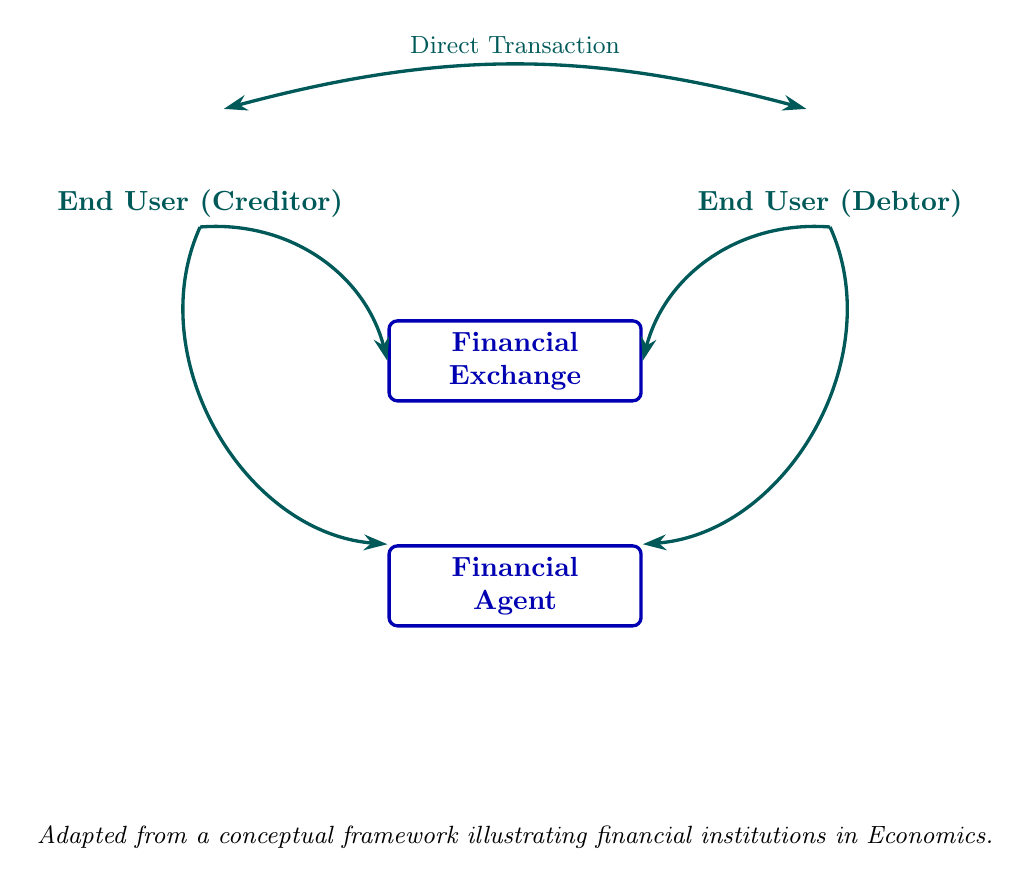
\begin{tikzpicture}[
    >=Stealth,
    node distance=1.8cm,
    font=\rmfamily,
    box/.style={
        draw=blue!70!black,
        very thick,
        rounded corners=3pt,
        inner sep=4pt,
        minimum width=3.2cm,
        minimum height=0.9cm,
        align=center,
        text=blue!70!black,
        font=\bfseries
    },
    flow/.style={
        -{Stealth[length=3mm,width=2mm]},
        very thick,
        draw=teal!70!black
    }
]

% Positions
\node[text=teal!70!black, font=\bfseries] (cred) at (-4,2) {End User (Creditor)};
\node[text=teal!70!black, font=\bfseries] (debt) at (4,2) {End User (Debtor)};

\node[box] (exchange) at (0,0) {Financial\\Exchange};
\node[box, below=1.8cm of exchange] (agent) {Financial\\Agent};

% Direct transaction arrow (top)
\draw[very thick, draw=teal!70!black, {Stealth[length=3mm,width=2mm]}-{Stealth[length=3mm,width=2mm]}] ($(cred.north)+(0.3,0.9)$) 
  to[bend left=15] node[above,sloped,pos=0.5,font=\small,text=teal!70!black] {Direct Transaction} 
  ($(debt.north)+(-0.3,0.9)$);

% Arrows from end users to Financial Exchange
\draw[flow] (cred.south) to[bend left=40] (exchange.west);
\draw[flow] (debt.south) to[bend right=40] (exchange.east);

% Arrows from end users to Financial Agent
\draw[flow] (cred.south) to[bend right=55] (agent.north west);
\draw[flow] (debt.south) to[bend left=55] (agent.north east);

% Caption
\node[below=2.4cm of agent, align=center, font=\itshape\small] 
{Adapted from a conceptual framework illustrating financial institutions in Economics.};

\end{tikzpicture}
\end{document}
